%%% LaTeX Template: Two column article
%%%
%%% Source: http://www.howtotex.com/
%%% Feel free to distribute this template, but please keep to referal to http://www.howtotex.com/ here.
%%% Date: February 2011

%%% Preamble
\documentclass[	DIV=calc,%
			paper=a4,%
			fontsize=11pt,%
			twocolumn]{scrartcl}					% KOMA-article class

\usepackage{lipsum}								% Package to create dummy text

\usepackage[english]{babel}							% English language/hyphenation
\usepackage[protrusion=true,expansion=true]{microtype}			% Better typography
\usepackage{amsmath,amsfonts,amsthm}					% Math packages
\usepackage[pdftex]{graphicx}							% Enable pdflatex
\usepackage[svgnames]{xcolor}							% Enabling colors by their 'svgnames'
\usepackage[hang, small,labelfont=bf,up,textfont=it,up]{caption}	% Custom captions under/above floats
\usepackage{epstopdf}								% Converts .eps to .pdf
\usepackage{subfig}								% Subfigures
\usepackage{booktabs}								% Nicer tables
\usepackage{fix-cm}								% Custom fontsizes



%%% Custom sectioning (sectsty package)
\usepackage{sectsty}								% Custom sectioning (see below)
\allsectionsfont{%									% Change font of al section commands
	\usefont{OT1}{phv}{b}{n}%						% bch-b-n: CharterBT-Bold font
}

\sectionfont{%									% Change font of \section command
	\usefont{OT1}{phv}{b}{n}%						% bch-b-n: CharterBT-Bold font
}



%%% Headers and footers
\usepackage{fancyhdr}								% Needed to define custom headers/footers
\pagestyle{fancy}								% Enabling the custom headers/footers
\usepackage{lastpage}	

% Header (empty)
\lhead{}
\chead{}
\rhead{}
% Footer (you may change this to your own needs)
\lfoot{\footnotesize \texttt{ECS 272} \textbullet ~Visualization}
\cfoot{}
\rfoot{\footnotesize Page \thepage\ of \pageref{LastPage}}		% "Page 1 of 2"
\renewcommand{\headrulewidth}{0.0pt}
\renewcommand{\footrulewidth}{0.4pt}



%%% Creating an initial of the very first character of the content
\usepackage{lettrine}
\newcommand{\initial}[1]{%
     \lettrine[lines=3,lhang=0.3,nindent=0em]{
     				\color{Black}
     				{\textsf{#1}}}{}}



%%% Title, author and date metadata
\usepackage{titling}								% For custom titles

\newcommand{\HorRule}{\color{Black}%					% Creating a horizontal rule
\rule{\linewidth}{1pt}%
}
%%begin novalidate
\pretitle{\vspace{-30pt} \begin{flushleft} \HorRule 
\fontsize{50}{50} \usefont{OT1}{phv}{b}{n} \color{Black} \selectfont 
}
\title{Outlier-preserving Focus and Context Visualization for Parallel Coordinates}		% Title of your article goes here
\posttitle{\par\end{flushleft}\vskip 0.5em}

\preauthor{\begin{flushleft}
\large \lineskip 0.5em \usefont{OT1}{phv}{b}{sl} \color{Black}}
\author{Vincent Yang, Bradley Wang }			% Author name goes here
\postauthor{\footnotesize \usefont{OT1}{phv}{m}{sl} \color{Black} 
					University of California, Davis 		% Institution of author
\date{}										% No date
\par\end{flushleft}\HorRule}
%%end novalidate



%%% Begin document
\begin{document}
\maketitle
\thispagestyle{fancy} 								% Enabling the custom headers/footers for the first page 


\section {Goal and Approach}
Our goal in this project was to create a parallel coordinates system that would make outliers and primary trends extremely obvious for the viewer. The system should scale well with large datasets and be an effective tool for finding interesting relationships or outliers. This would allow us
to scale with large datasets.

As for personal goals, this is our first time implementing a visualization paper, so we
hope to learn about what goes into a research paper furthering visualization. 
Thus far in class, we have only seen the end results and learned about using others' tools,
but haven't created our own. 

Our approach is to for precompute the data we need. This would involve (a) binning the data, (b) figuring out 
where the main trends are, (c) figuring out where the outliers are, and (d) figuring out where the clusters are. 
For binning the data, we will look at every combination of 2 axes just as they specify in the paper. Of each pair,
we will create a table of bins representing the frequency of certain bin combinations. With these, we will take the
more populated bins and call them our trends, then finding the outliers by using median and isolation filters.

Clustering will involve using gaussian smoothing then iteratively moving from more populated bins
to less populated bins to determine where interesting clusters might lie. 

Once we have precomputed this data, we will plot it on our system with d3 and webgl. d3 creates
the axes and labels, and supports the ability to move axes around. Webgl will display our polygons for
representing trends as well as drawing the outliers. This would also take care of the textures for us. 

To run the precomputing script on data.csv with 10 bins per axis, run \texttt{python3 bin.py data 10}. The input
data should have no quotes and end in \texttt{.csv}. This will also create array.png and array2.png. These show examples of the 
data before and after gaussian filtering. 

\begin{figure}
  \caption{Our Implemented System}
  \centering
    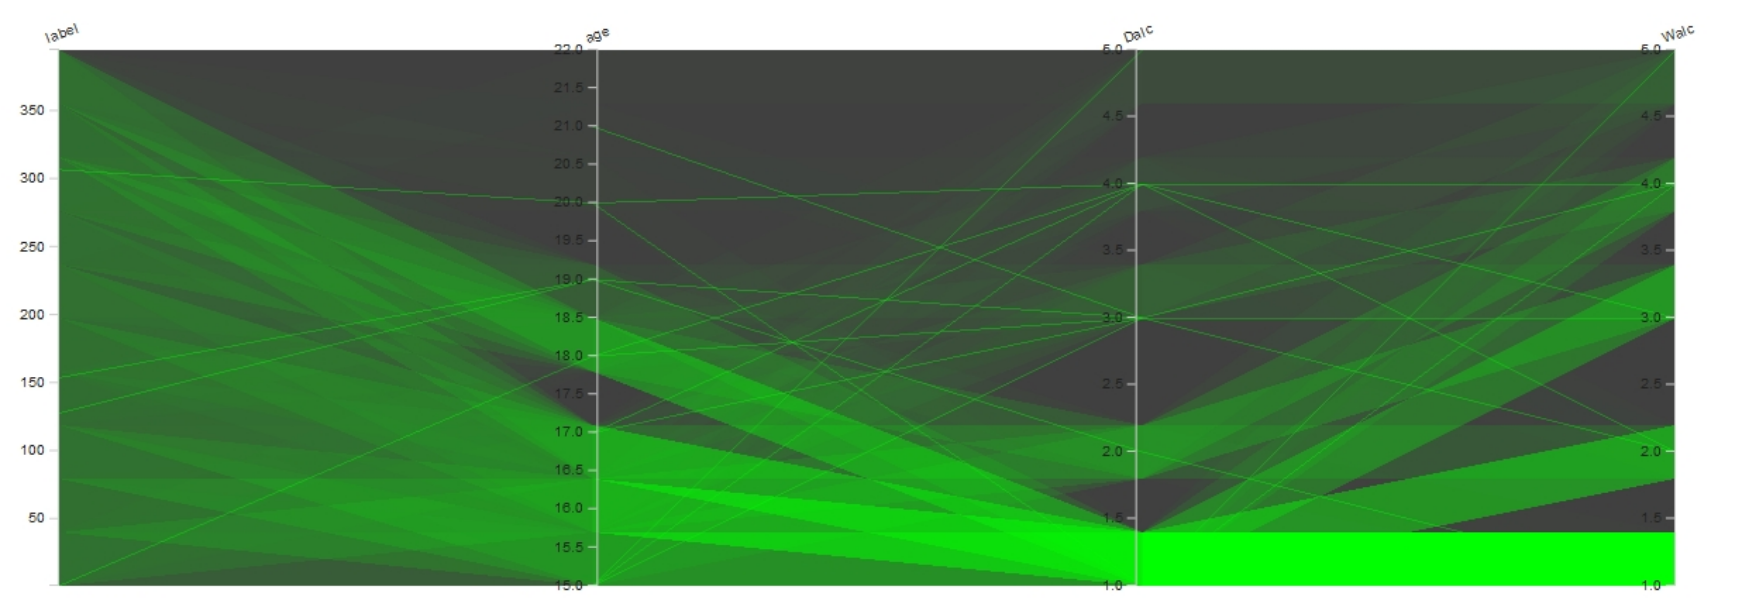
\includegraphics[width=9cm]{alc-opf.png}
\end{figure}

\begin{figure}
  \caption{Traditional Parallel Coordinates}
  \centering
    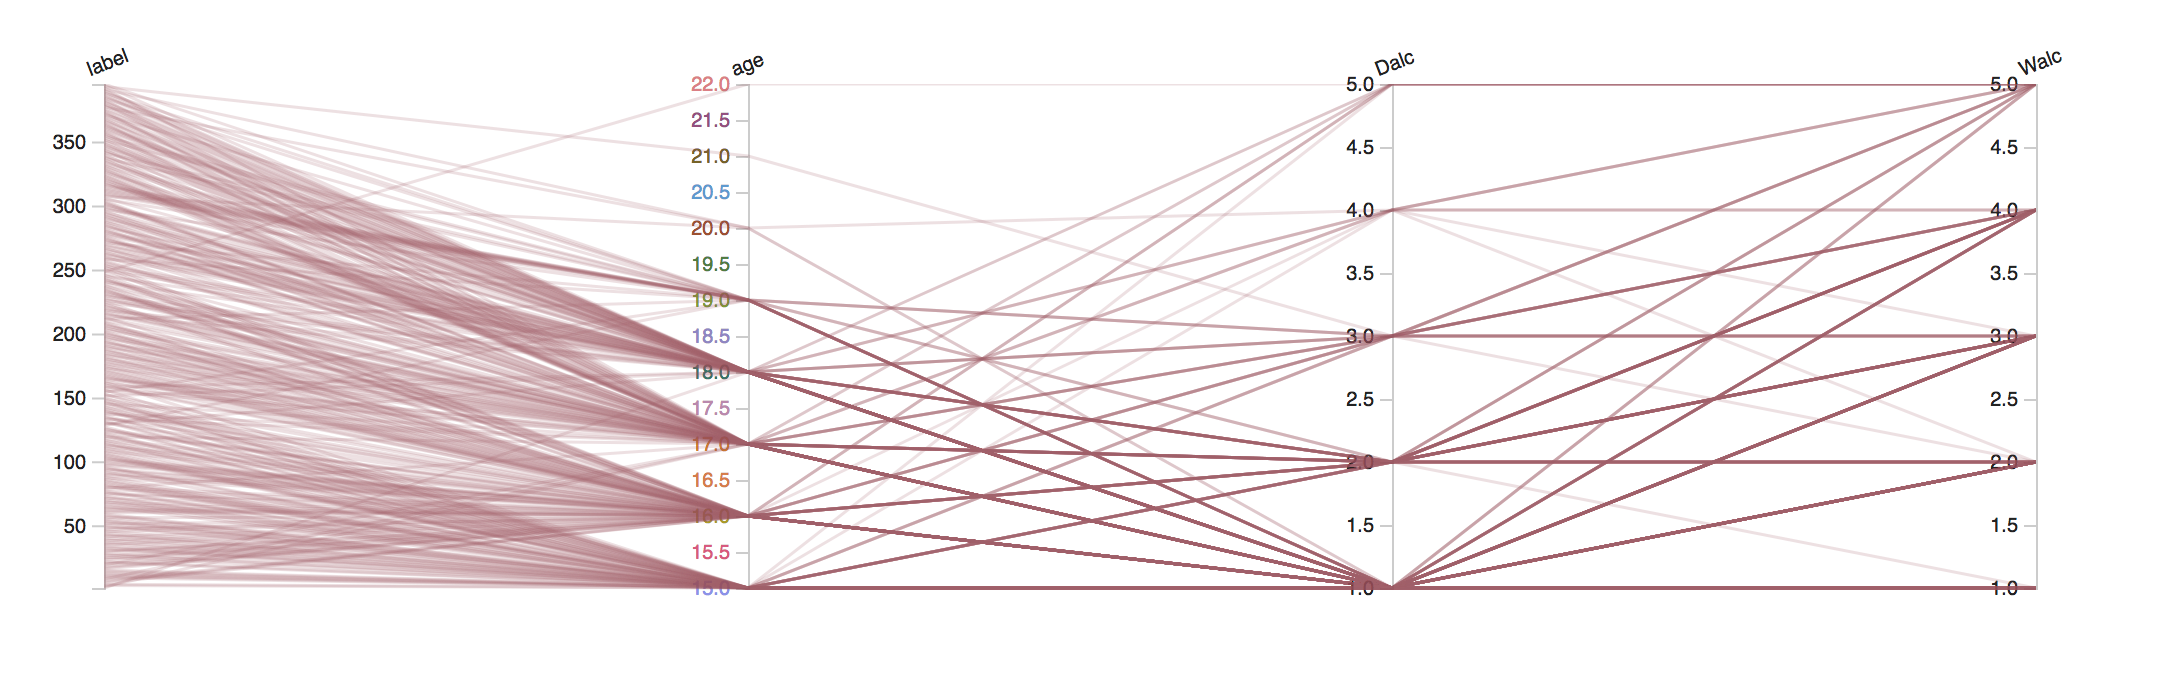
\includegraphics[width=9cm]{age-alc-orig.png}
\end{figure}

From these pictures, we can see the difference between our implemented system and a traditional
parallel coordinates plot. Even on a small dataset with only several hundred rows, 
it is easier to notice on the lower right that there are many people in lower ends of both Dalc and Walc. 

We can also find the outliers easier, which are clearly in the upper right for our implemented system. 
It is difficult to see the difference between outliers and trends in conventional parallel coordinates.

\section {Our Experience}

\subsection {Positives}
This paper was interesting because it has a new approach to parallel coordinates that we haven't seen before. This was also our first time implementing a visualization paper, 
which gave us insight into how difficult it is to create these systems. Far more effort went into figuring out how to use which tools, which I didn't expect. Next, the paper's approach
and pictures also gave us a strong idea on the benefits of their method. I learned alot on how data may be processed before displaying to the user. We also learned about
how people in visualization have to think about the reality of their visualization methods -- that computing might take a long time or the screen might not be large enough. 

\subsection {Negatives}
We found the paper quite difficult to make sense of. The title of the paper implied that it would focus on outlier and focus, but it didn't distinguish the difference between outlier and focus particularly well. This made working on the implementation rather difficult, as we had to read significantly more background literature than previously expected. 
We also found that the paper was somewhat misleading. It promotes efficiency via calculating bucket frequency to accentuate features with parallel coordinates plots. A large part of the paper focuses on the speed benefits of this approach. They also mention that buckets should be calculated between pairs of axes, implying that you would only need to calculate $n-1$ axes pairs where $n$ is the number of axes. However, this is not true at all. Later on in the paper, they bring up the point that if you actually want to be able to reorder the axes (a common feature in parallel coordinates), then you would have to calculate frequencies for every possible combination of axes. This is far more than before! With this, we lose much of the speedup we previously obtained with their method. 
Initially, we implemented the preprocessing by using JavaScript, but found that using Python to precompute the buckets as opposed to computing on page-load made far more sense for the user. With this, the user could simply load data as opposed to processing then loading. 
Some challenges I faced with precomputing was figuring out how to use gaussian smoothing. In the paper, they simply mentioned that it was a common technique in visualization then linked to an early paper regarding gaussian smoothing. This helped very little with my understanding for what to do. I ended up finding blog posts teaching me how to do 2D gaussian smoothing. In the current implementation, we had to look at various smoothnesses dataset by dataset to determine which alpha value (how much to smooth) for each dataset. From what we could find, the proper value should be the standard deviation. Yet with many datasets, we would get completely uniform data, making the data too smooth. In their implementation, they likely found a better way to run smoothing for displaying/calculating the focus. 
Another issue with focus is that they never described how the user would interact with their system to specify which areas to focus on. In traditional parallel coordinates, the user may “scrub” an axis to indicate that they want to look at a subset of data where the values are within a certain range on a given axis. Yet in this implementation, this functionality doesn't seem to work -- rendering the original values for the user to see would somewhat defeat the purpose of displaying trends and outliers for extremely large datasets. Scrubbing for finding trends or outliers doesn't make sense either, since the user should already be able to see this clearly. 

\section {System Differences}
Our implementation allows for the user to specify how many bins they want. The paper doesn't cover details of how the user interacts with their system, so we decided to simply add a command line argument to the precomputation script. This is accessible by running python3 bin.py n, where n is the number of bins desired per axis. 
Bradley talk about alpha blending here. 

Our implementation also has axis labels so the user can see exactly where trends/outliers lie. In their implementation,
they have labels at the very top and bottom, but nowhere in between. 

They discuss using the GPU to optimize rendering, but we don't interact with the GPU. We wanted to focus on 
getting a working implementation and observing the benefits of binning. 


\subsection {Datasets Chosen}
The paper's examples used a CFD simulation dataset (mixture of two fluids) and remote sense data. We were unable to find the original datasets, which made it difficult for us to compare our implementations. 
We chose the international census data to emphasize the speed improvements with their method. The census data is nearly a gigabyte and has over 100 axes, which makes it interesting for us to observe. This dataset was released by the US Census Bureau in 1950 and has its projections through to 2050. Specifically, the original data used to generate this dataset came from observing cities with over 5000 people. We looked specifically at midyear population age by country. 
Our other datasets are smaller. As the number of axes increased, we had a drastic increase in time spent computing. However, with adding more rows, we didn't observe a similar slowdown. This is likely because adding values to buckets runs in linear time but adding an axis requires that we calculate more buckets for every existing axis. \\

For all of our datasets, we made sure to either choose datasets without numerical categorical variables or to remove those columns. Some useful work that could be done here would be to
map categorical variables to regular intervals, but this would not work well with their approach of creating trends, as the order of the trends would have no inherent importance
but this would affect our trend detection. Because of this, it seems the specific usecase for their approach is actually quite small. 

The list of datasets we chose are BudgetFood, EuStockMarkets, and MidyearPopulationCensus. The largest dataset is MidyearPopulationCensus, which is over 800 mb. We
cleaned out all of the datasets by converting male/female values to 0 and 1, and removing non-numerical columns. 

\section {Case Study/Analysis Results}
\begin{tabular}{ |p{2cm}||p{1cm}||p{1cm}||p{1.2cm}|  }
 \hline
 \multicolumn{4}{|c|}{Time in Sec.} \\
 \hline
 Data& Orig. Time& Our Time & Rows\\
 \hline
 creditdefault& 13 & 8 & 10001\\
 quakes&   3 & 10 & 1001\\
 census &- &32min & 3058281\\
 EuStock &3.1 &8 & 1861\\
 age-alc &$<1$ &$<1$ & 396\\
 \hline
\end{tabular}

The strength of this system is clearly shown in the census data. With the normal 
parallel coordinates implementation, the d3 couldn't even handle holding the data in 
memory and threw an allocation size overflow error. Admittedly, this dataset also
took over half an hour to precompute. The long precomputing time is likely due to
the high number of axes -- there are over 100 axes in this dataset, meaning 
our precomputation calculated $100^2$ possible combinations of axes. 

With most of the small datasets of only several thousand rows, rendering the data
was extremely quick with traditional parallel coordinates. This is as expected, as 
there is minimal improvement, if any, from counting frequencies when there isn't much to draw anyway. 


\section {Strengths and Limitations}
A key strength of this method is that there is far less data to plot at a time. When we tried to render traditional parallel coordinates with some gigabyte datasets, it took almost a minute just to load all of the data onto
the browser, then more to draw. Although it took a while to precompute our implementation, it rendered far faster. Additionally, it would be fully possible to parallelize our
precomputation to enable the user to spend even less time in this step. 

As we can see in this image, it is rather difficult to make sense of what is in the original data, as
there are so many data points on the right. This is the credit default dataset, which shows
the attributes of people who default or don't default on their credit card payments. Just rendering
this dataset which has 10,000 lines takes around 12 seconds. 
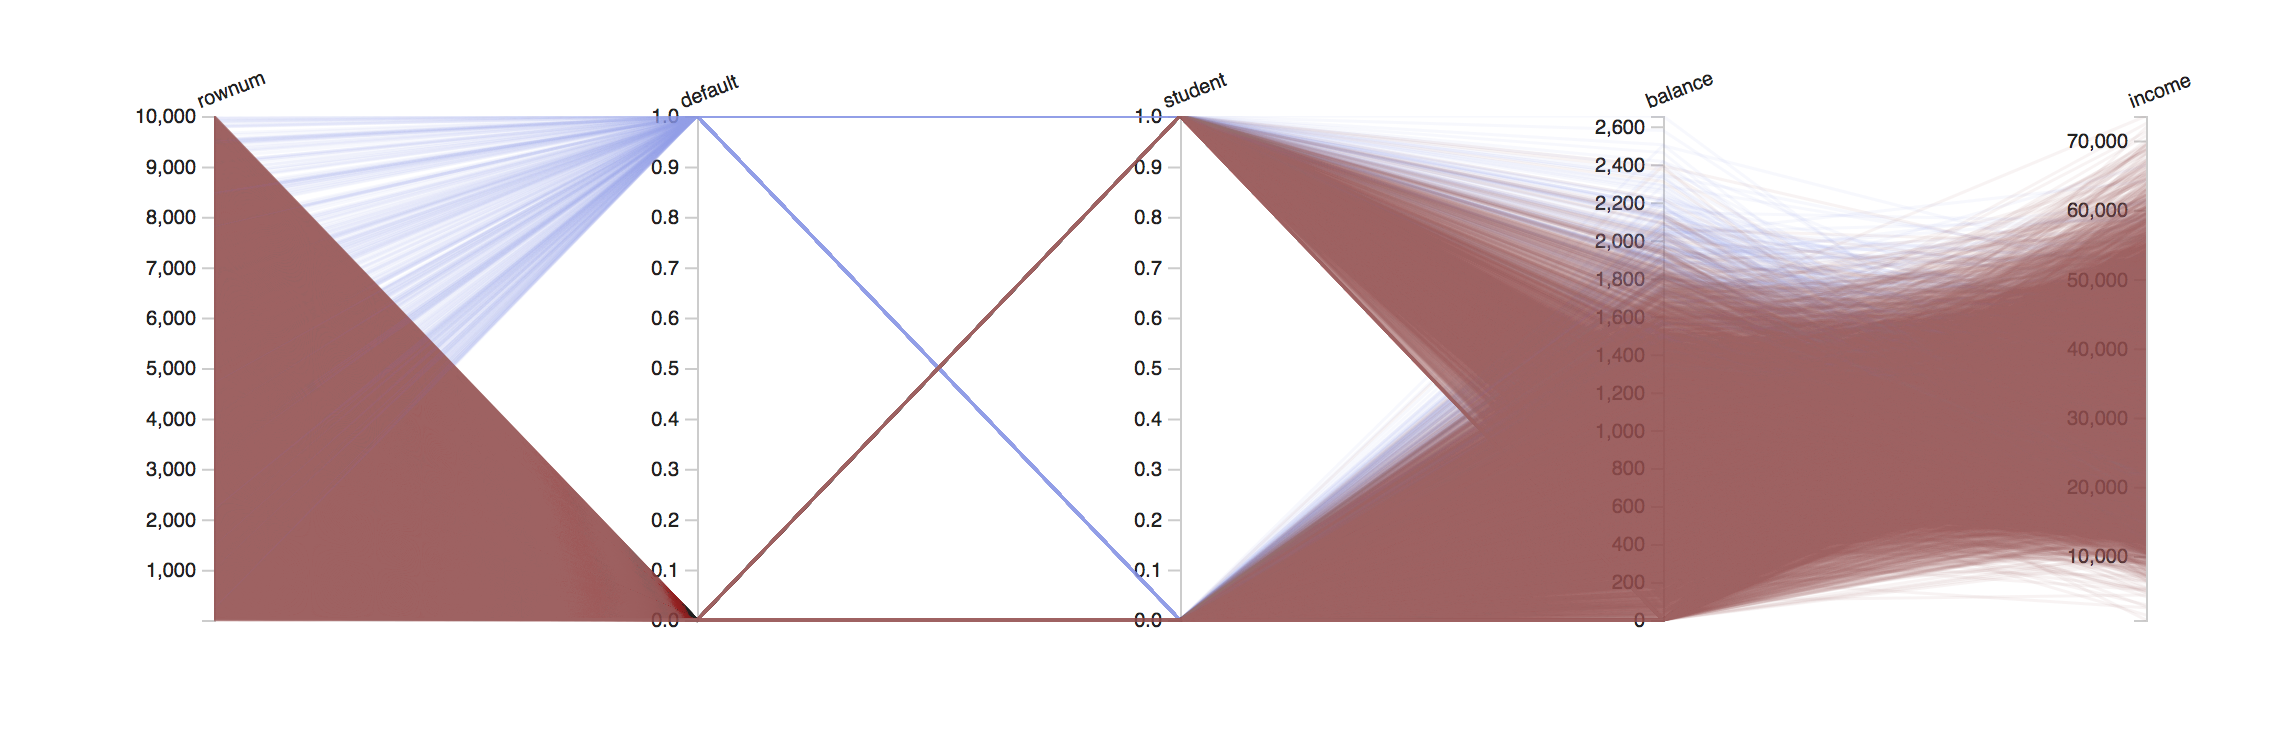
\includegraphics[width=9cm]{credit-default-parcoord.png}

A limitation of this method and parallel coordinates overall is that it is primarily designed for numerical variables. As such, we can't work with many datasets. We also can't represent time series or continuous data well, since we bind them to their closest bucket ranges. 
This work could be furthered by diving deeper into how buckets should be created. Bucket creation is core to their paper and may drastically affect the visualization. We defaulted to using 10 buckets per axis, but this may result in a loss of detail for the final visualization. 
Another idea for future work would be to improve the outlier detection. The outlier detection works by scanning buckets that are at least 10\% full. Changing this barrier would change the outliers visible for the user. 


% Including the bibliography
\bibliographystyle{plain}
%\nocite{*}
\bibliography{paper}
\end{document}
